% \section{Analysis}

\section{Task Error Analysis}
% \begin{figure*}
    \centering
    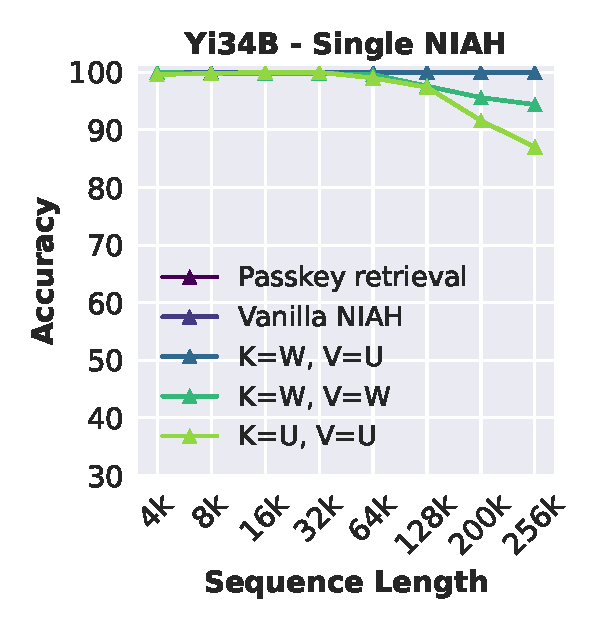
\includegraphics[width=0.24\linewidth]{Image/pdf/Yi_SNIAH.pdf}
    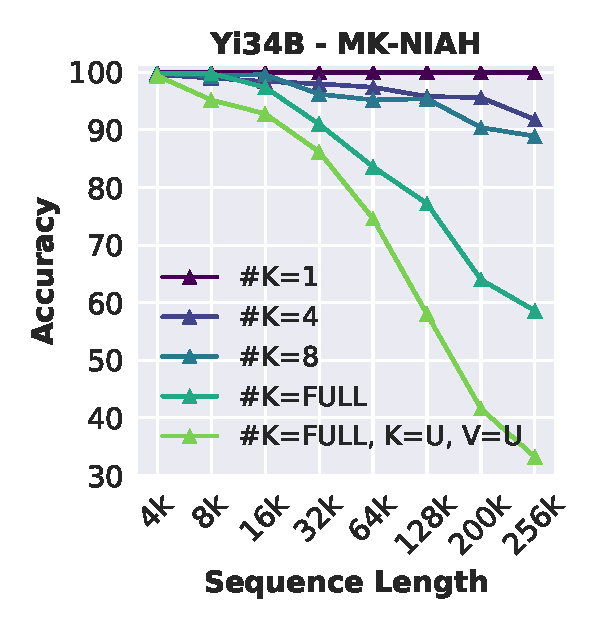
\includegraphics[width=0.24\linewidth]{Image/pdf/Yi_MKNIAH.pdf}
    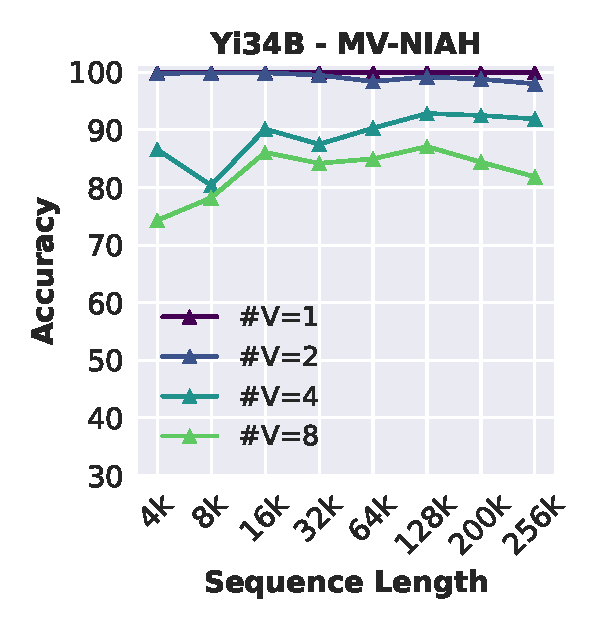
\includegraphics[width=0.24\linewidth]{Image/pdf/Yi_MVNIAH.pdf}
    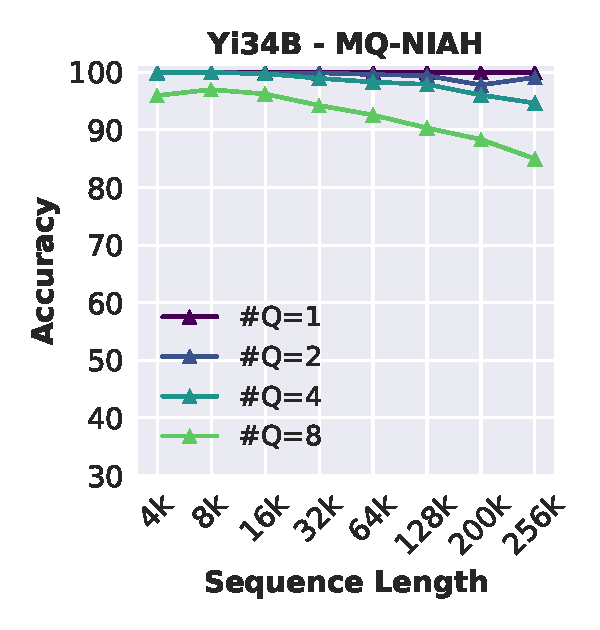
\includegraphics[width=0.24\linewidth]{Image/pdf/Yi_MQNIAH.pdf}
    \caption{Performance of Yi-34B in the needle-in-a-haystack (NIAH) tasks. By default, we use word-number as the key-value pair and Paul Graham essays as the haystack. Yi is not robust to the change of needle types and degrades with the increasing amount of distractors. (W: words; N: numbers; U: UUIDs; Full: entire haystack).}
    \label{fig:yi_niah}
\end{figure*}
We evaluate Yi-34B-200K with increased input lengths (up to 256K) on more complex tasks to understand the effect of task configurations and failure modes on \ruler.
% 
\paragraph{Non-robustness to ``needle'' types.} Figure~\ref{fig:yi_niah} (left) shows that while Yi achieves almost perfect performance when using needle of word-number pair in the standard passkey retrieval and vanilla NIAH, performance degrades when the needle takes other forms. We observe the largest degradation in the task of retrieving UUIDs, for which Yi sometimes fail to return the complete 32 digits given long ($>$128K) input context.

\paragraph{Failure to ignore distractors.}   Figure~\ref{fig:yi_niah} (middle-left) shows that increasing the number of distracting needles steadily lowers performance, with Yi dropping by $\sim$40 points at 256K in the extreme version, where the context is full of irrelevant needles ({\small \#K=FULL}). Error analysis reveals that Yi fails to effectively ignore the hard distractors given long input context, thus incorrectly retrieves values associated with the distractor keys. In the extreme version, Yi often returns values from the vicinity of the target, suggesting coarse match of the range but the lack of precision to locate the key when the target is in-distribution of the noises.

\paragraph{Return incomplete information.} Consistent with previous works~\citep{lwm, gemini}, we notice significant degradation in performance when the model needs to retrieve multiple items from a long input. For instance, increasing the number of queries from 1 to 8 drops the performance by $\sim$15 points (Figure~\ref{fig:yi_niah} right). When the model needs to retrieve multiple values associated with the same key (Figure~\ref{fig:yi_niah} middle-right), Yi often outputs duplicated answers without returning the complete set of values, implying uneven associations between the key and each of its values.
\begin{figure*}
    \centering
    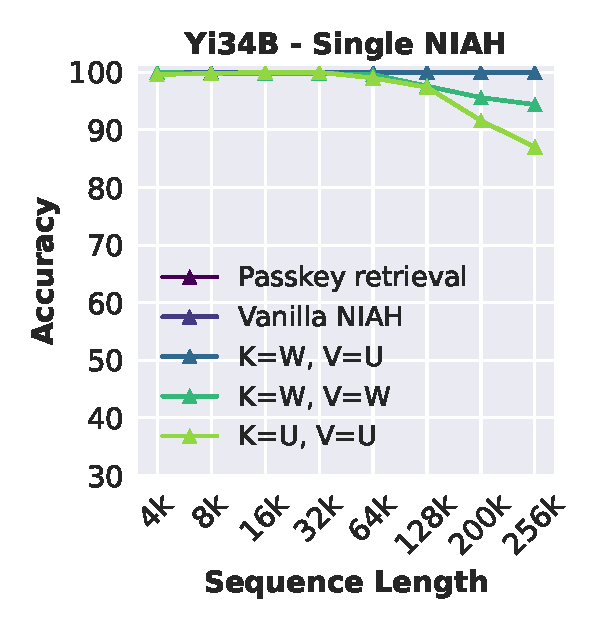
\includegraphics[width=0.24\linewidth]{Image/pdf/Yi_SNIAH.pdf}
    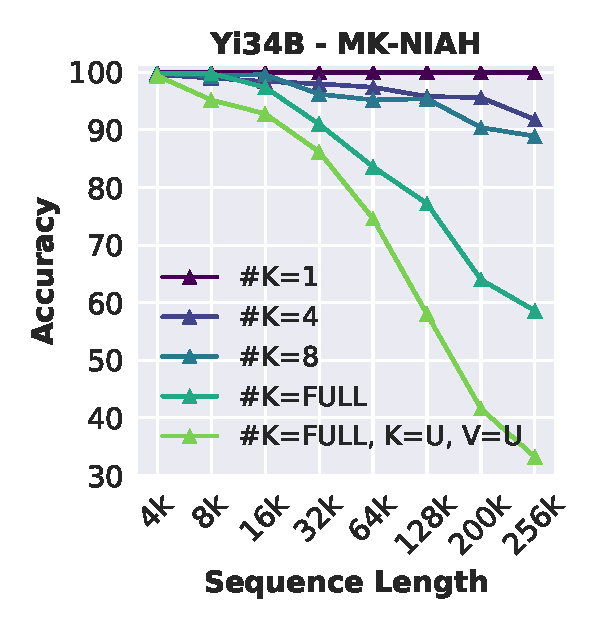
\includegraphics[width=0.24\linewidth]{Image/pdf/Yi_MKNIAH.pdf}
    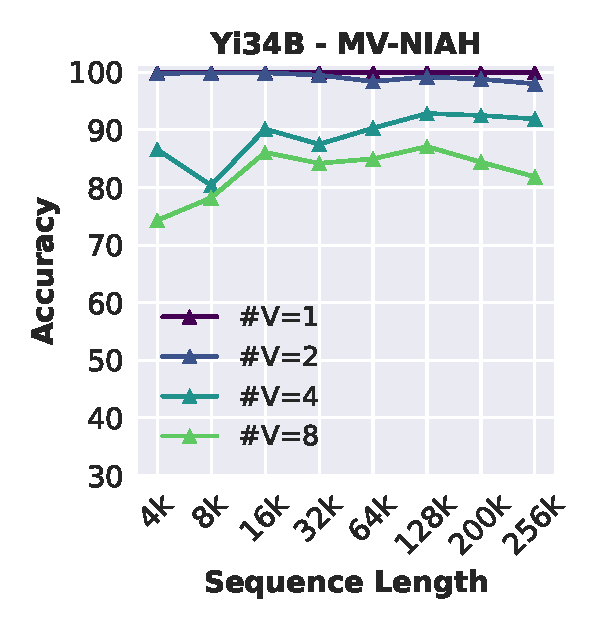
\includegraphics[width=0.24\linewidth]{Image/pdf/Yi_MVNIAH.pdf}
    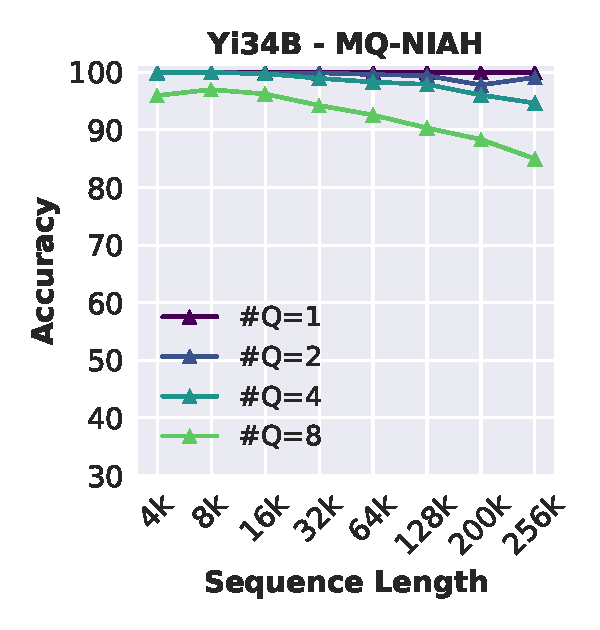
\includegraphics[width=0.24\linewidth]{Image/pdf/Yi_MQNIAH.pdf}
    \caption{Performance of Yi-34B in the needle-in-a-haystack (NIAH) tasks. By default, we use word-number as the key-value pair and Paul Graham essays as the haystack. Yi is not robust to the change of needle types and degrades with the increasing amount of distractors. (W: words; N: numbers; U: UUIDs; Full: entire haystack).}
    \label{fig:yi_niah}
\end{figure*}
\begin{figure*}
    \centering
    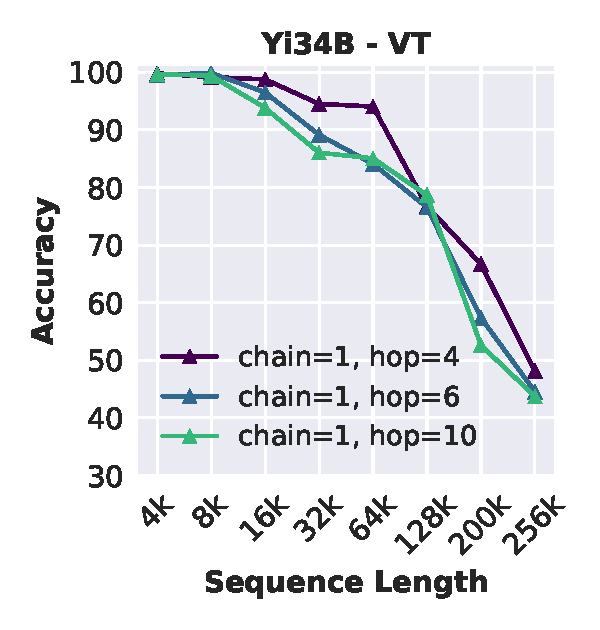
\includegraphics[width=0.24\linewidth]{Image/pdf/Yi_VT_1.pdf}
    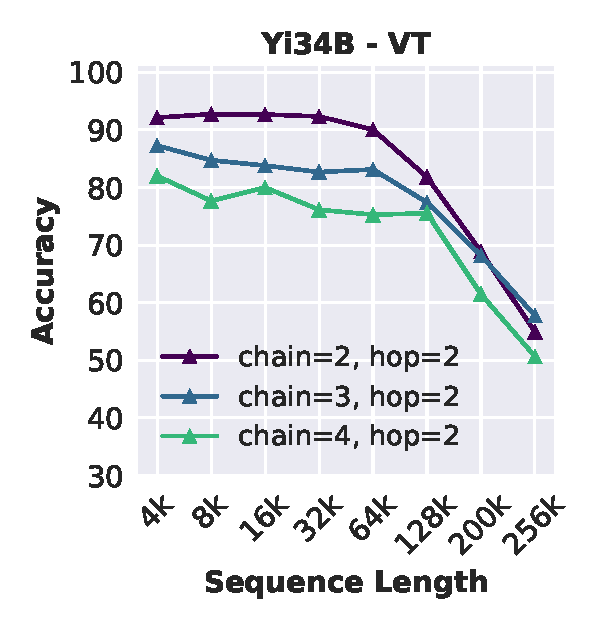
\includegraphics[width=0.24\linewidth]{Image/pdf/Yi_VT_2.pdf}
    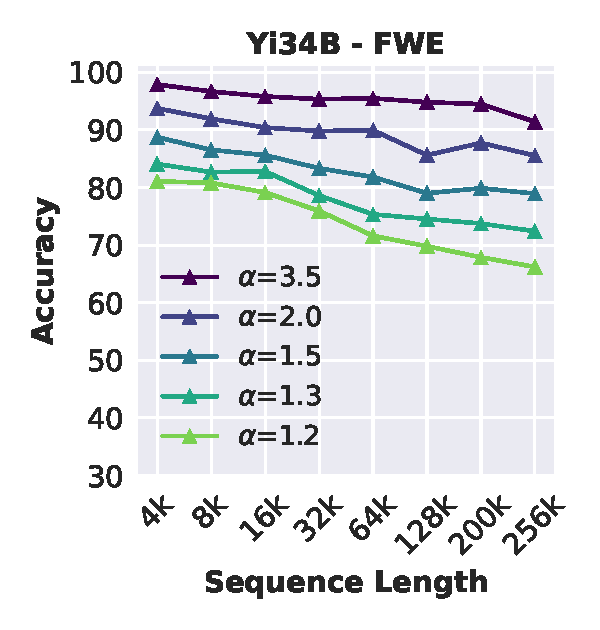
\includegraphics[width=0.24\linewidth]{Image/pdf/Yi_FWE.pdf}
    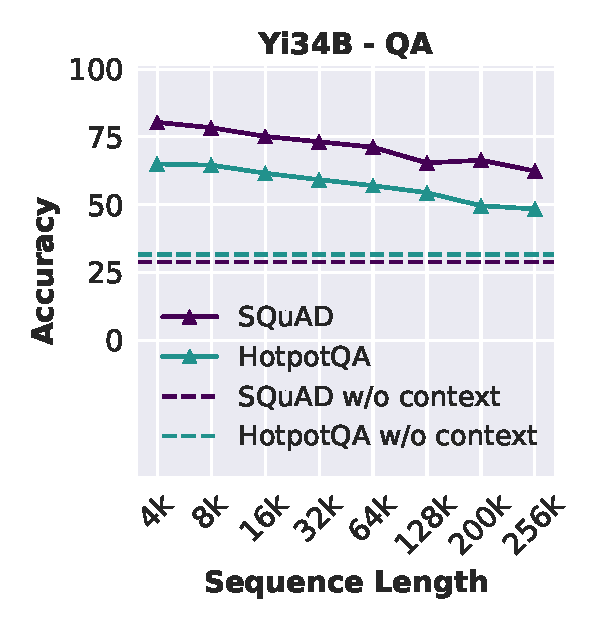
\includegraphics[width=0.24\linewidth]{Image/pdf/Yi_QA.pdf}
    \caption{Performance of Yi-34B in variable tracking (VT), frequent words extraction (FWE), and QA tasks across different task complexities. Yi shows large degradation and distinct trends with scaled context size in these non-retrieval tasks, demonstrating the need to evaluate behavior beyond retrieval from context.}
    \label{fig:yi_vt_fwe_qa}
\end{figure*}

\paragraph{Tendency to copy from context.} We notice that Yi has a strong tendency to copy from context verbatim when scaling the input length. This tendency is most notable in \emph{variable tracking} (VT) and \emph{common words extraction} (CWE) where we include one in-context demonstration at the beginning of the sequence. Over 80\% of Yi's output in the CWE task at 128K is simply a string copied from the one-shot example, whereas the copying is nonexistent for short sequences. \footnote{We also experimented with removing the one-shot example. The model will simply copy the string of the beginning of the input, likely due to the attention sinks~\citep{streemllm}.} This copying behavior is also present in the LWM model and LongAlpaca, however it is less prevalent in other models, such as Mixtral. This finding further reinforces the need to test behaviors other than retrieval given long input context.

\paragraph{Unreliable tracking within context.} For the \emph{variable tracking} task, both adding more chains and more hops contribute to large degradation in Yi's performance. Yi consistently degrades in the more-hops setting as we increase context size (Figure~\ref{fig:yi_vt_fwe_qa} left), whereas the degradation in the more-chains setting is most significant for lengths greater than 128K (Figure~\ref{fig:yi_vt_fwe_qa} middle-left). Besides the aforementioned copying issue, Yi makes errors due to incorrectly returning empty strings or variables from other chains, implying a lack of ability to reliably trace the same entity within long context. These errors are also frequently observed in models that do not exhibit the copying behavior.

\paragraph{Failure to accurately aggregate.} We observe two common failure modes in aggregation tasks: incorrect use of parametric knowledge and inaccurate aggregation. Models that do not exhibit the copying issue in the CWE task, sometimes ignore the contextual information and instead use parametric knowledge to answer the query, especially at large context sizes. For instance, Mistral (7b-instruct-v0.2) returns high frequency words, such as ``the'', ``an'', ``a'', as output without counting the words in context. For the FWE task which demonstrates less the copying issue, Yi fails to correctly output the top frequent words as we decrease the $\alpha$ in Zeta distribution (Figure~\ref{fig:yi_vt_fwe_qa} middle-right). Decreasing $\alpha$ leads to smaller difference in frequency among words, increasing the difficulty to distinguish the top-frequent words.

\paragraph{Frequent hallucination in long-context QA.} For the QA tasks, Yi's performance approaches its no-context baseline as we extend the context with distracting paragraphs (Figure~\ref{fig:yi_vt_fwe_qa} right). The degradation stems primarily from hallucination and reduced reliance on contextual information. We notice that, at large context sizes, model predictions sometimes are irrelevant to the question and can coincide with the answers of its no-context baseline. The overall worse performance in QA tasks confirms that the fuzzy matching between a query and a relevant paragraph in long context is a more challenging setting than the simplistic NIAH tests, where keys can be exactly located in context.
% as we extend context, we observe more freqeunt (1) hallucination and (2) reliance on  parametric knowledge 

% \paragraph{Question Answering}
% While our complexity of QA tasks is determined by dataset selection, we only observe a performance shift across all lengths in Figure~\ref{fig:yi_vt_fwe_qa} when comparing single-hop (SQuAD) and multi-hop (HotpotQA) datasets. 
% Furthermore, we assess performance using only the question without any contextual information to evaluate the influence of parametric knowledge. The findings indicate that the performance degradation with long-context may fall below the no-context baseline in realistic tasks.

% \paragraph{Lost in the middle}\sscomment{model performance v-shape when putting needle at various positions} (cheng-ping squad: LWM Yi; from which length lost in the middle becomes severe)

% \paragraph{Task Comparison} \sscomment{model case study?? similar avg perf by large variations by categories}


\section{Model Analysis} \label{sec:mdl_analysis}
\begin{figure*}
    \centering
    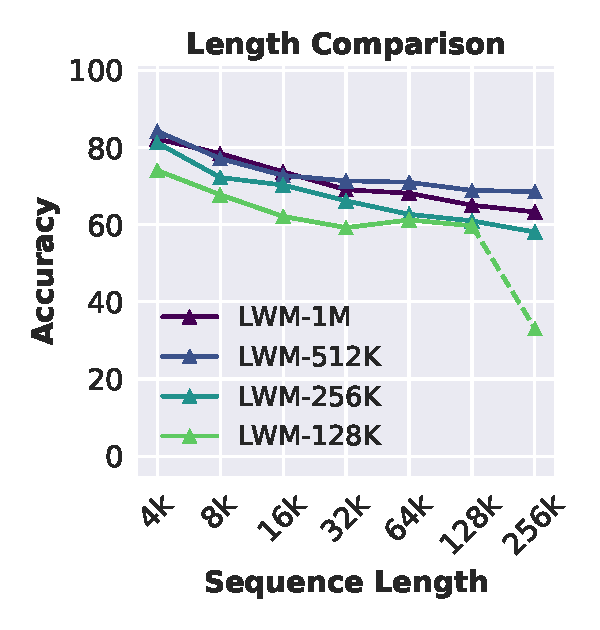
\includegraphics[width=0.24\linewidth]{Image/pdf/LWM.pdf}
    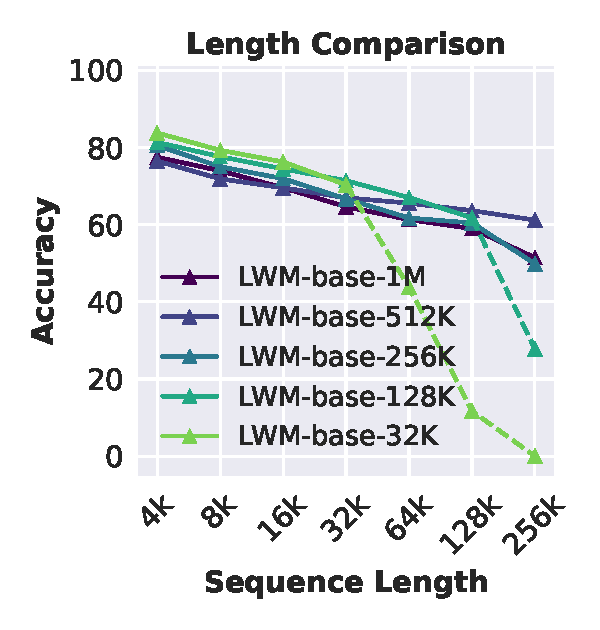
\includegraphics[width=0.24\linewidth]{Image/pdf/LWM-base.pdf}
    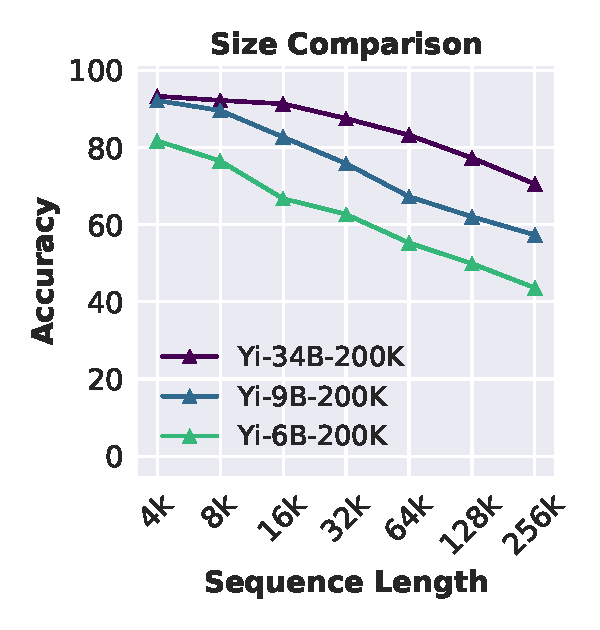
\includegraphics[width=0.24\linewidth]{Image/pdf/Yi.pdf}
    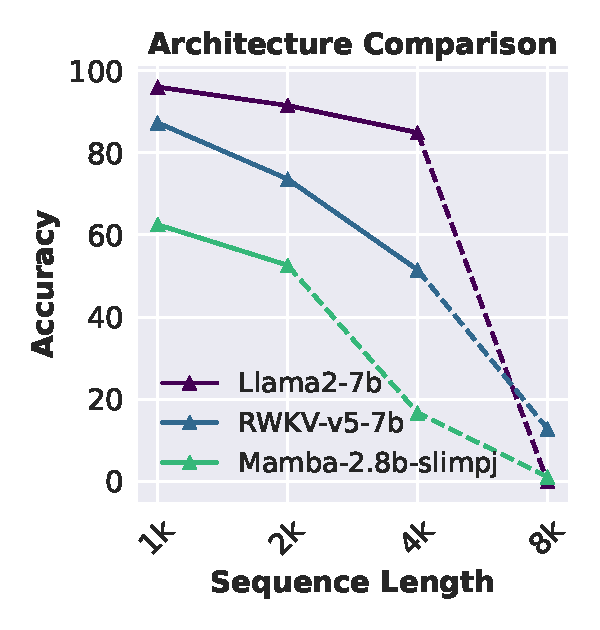
\includegraphics[width=0.24\linewidth]{Image/pdf/MambaRWKV.pdf}
    
    \caption{(\textbf{Left \& middle left}): Comparison of LargeWorldModel (LWM) series trained up to various context sizes with fixed parameter size of 7B. (\textbf{Middle right}): Comparison of Yi suite models with different parameter sizes with controlled training context length of 200K. (\textbf{Right}): Performance of non-Transformer architectures lags behind the Transformer baseline Llama2-7B by large margin. Length extrapolation is presented with dashed lines.}
    \label{fig:lwm_yi}
\end{figure*}

\paragraph{Effect of training context length.} Do models trained with larger context sizes perform better on \ruler? We evaluate the suite of LargeWorldModels~\citep[][LWM]{lwm} of equal parameter size and trained up to various context lengths. Figure~\ref{fig:lwm_yi} (left \& middle-left) shows that larger context sizes overall lead to better performance, but the ranking can be inconsistent for long sequences. For instance, the model trained with 1M context size (LWM-1M) is worse than the one with 512K at length of 256K, likely due to insufficient training for adjusting to the new base frequency in RoPE. Moreover, we observe abrupt performance drops when models need to extrapolate to unseen lengths (e.g., LMW-128K given input of 256K), and almost linear degradation with input length on log scale within the max training context size.
% , below the max training context size.
% \vspace{-0.93em}
\paragraph{Effect of model size} The top models in our main results are much larger than other models. To ablate the effect of model size, we evaluate Yi-34B-200k, Yi-9B-200k, and Yi-6B-200k, all trained up to the same context length using the same data blend. Figure~\ref{fig:lwm_yi} (middle-right) shows that the 34B model is significantly better than the 6B model on \ruler~for both performance at length of 4K and the relative degradation, suggesting the benefit of scaling model sizes for better long-context modeling.
% \vspace{-0.93em}
% \begin{table}[!h]
\centering
\footnotesize
\begin{tabular}{@{}lccccc@{}}
\toprule
                               & 1k             & 2k    & 4k    & 8k  & 16k \\ \midrule
\textbf{noise k: words 1 v: numbers 1 r: 1} & 100.0 & 100.0 & 100.0 & 0.0 & 0.0 \\
\textbf{k: uuids $\infty$ v: uuids 1 r: 1}   & 4.6      & 0.0   & 0.0   & 0.0 & 0.0 \\
\textbf{book k: words 1 v: uuids 1 r: 1} & 100.0   & 99.4  & 0.2   & 0.0 & 0.0 \\
\textbf{variable\_tracking\_2\_2}    & 32.9   & 36.2  & 1.9   & 0.0 & 0.0 \\
\textbf{frequent word extraction alpha=3.5} & 81.5 & 81.9  & 54.5  & 1.0 & 0.0 \\ \bottomrule
\end{tabular}
\caption{Select task performance of Mamba-2.8B-slimpj. Mamba  }
\label{tab:mamba_result}
\end{table}

\paragraph{Effect of architecture}  We evaluate the effective context length for two models with non-Transformer architectures: RWKV-v5~\citep{rwkv} and Mamba-2.8B-slimpj~\citep{mamba}. We find that both models demonstrate significant degradation when extending context size to 8K, and both underperform the Transformer baseline Llama2-7B by large margins up till the length of 4K, beyond which Llama2 shows poor length extrapolation performance (Figure~\ref{fig:lwm_yi} right).


% Mamba can achieve perfect extrapolation in the simplest passkey retrieval task for sequencese up to 4k tokens; however, its performance drops to zero beyond 4k. For the task of retrieving uuid from books, Mamba shows approximately perfect result up till its training length, yet when noises take the same form as the needle (uuid $\infty$), Mamba fails to correctly recall the queried key, suggesting further room to improve its selection mechanism and the limited state space. Overall, considering its performance on other tasks, we conclude that state-space model currently lags behind Transformer-based models on our benchmark.


% \paragraph{Single NIAH} Based on the changes of different types of needle keys, needle values, and haystack, Figure~\ref{fig:yi_niah} (left) shows that passkey retrieval and vanilla NIAH obtain perfect scores while needles with full words and UUIDs can lead to performance degradation as the context sizes increase. Analyzing the failure of using word needles, we found model may ignore the context and \sscomment{what do you mean by explain the output with hallucination?} explain the output with hallucination because using words may confuse model with the parametric knowledge. For wrong predictions of UUIDs, model may copy the needle keys or response with the incomplete needle values, suggesting it is harder to retrieve a long span value with multiple tokens.
% Here is an incorrect example: \textit{The special magic word for \textbf{petite-superiority} mentioned in the provided text is \textbf{naughtiness.} This word is used to describe the quality of being naughty, which is associated with the concept of \textbf{petite-superiority}.}

% \paragraph{Multi-key NIAH} In Figure~\ref{fig:yi_niah} (middle left),  we observe that an increase in distracting needles can confuse our model to retrieve the correct one. The model struggles to ignore these distractors, particularly in scenarios where the haystack is filled with needles. Analyzing the wrong predictions, we find the model tend to output values in the vicinity of the correct needle keys, suggesting model pays attention to a broad context span rather than the specific details of key information. The comparison between S-NIAH and MK-NIAH reveals that the model is good at filtering out pure noise such as repeating sentences and essays, but faces challenges in effectively handling confusing distractions like needles. \sscomment{todo: mention the most challenging setting where needle is in-distribution of noises.}


% \paragraph{Multi-value and Multi-query NIAH}
% Both MV-NIAH and MQ-NIAH require the model to output multiple values during prediction.   Figure~\ref{fig:yi_niah} (middle right \& right) illustrates that as the number of needle values or queries increases, the model's performance drops because it needs to retrieve more tokens. Given this scenario, we find that the model begins to output incomplete or duplicated results. In MV-NIAH, there is even a significant degradation with Yi-34B at short context lengths, highlighting the challenge of retrieving multiple needles based on a single query compared to MQ-NIAH.

% \paragraph{Variable Tracking} Figure~\ref{fig:yi_vt_fwe_qa} \textbf{(left)} and \textbf{(middle)} show that increasing the number of chains and the number hops both lead to performance degradation as the context sizes increase. The large drop in performance at sequence of 4k tokens confirms that having additional distractor chains is a more challenging setting compared to simply increasing the number of hops with a single chain in context, since Yi can achieve rougly 100\% accuracy at 4k even when there are 10 hops. We observe that models output empty strings or copy the few-shot output more frequently when sequence is long. Other errors stem from not being able to return all variables along the chain or incorrectly returning variables from distractor chain(s). 

% \paragraph{Aggregation} 
% % \sscomment{todo: make it more concises} 
% We identify three main failure modes in aggregation tasks when scaling context sizes. 
% \textbf{(1)}. Relying on parametric knowledge:  In CWE, where we sample from real natural language word list, models such as Mistral-v0.2-instruct tend to return ``1. the 2. an 3. a $\dots$'' as the answer instead of extracting common words from the context. \textbf{(2)}. Copying few-shot output or the lead context: Over 80\% of the prediction of Yi34B and LWM-7B-chat in the CWE task, are simply copy of the few-shot example output when sequence length reaches 128k. However, the copying behavior is much less frequent at smaller context sizes, such as 4k. 
% % Further analysis is needed to understand these two models' shift in tendency from aggregation to retrieval when context sizes increase.
% \textbf{(3)}. Failing to correctly aggregate: for the cases where models do not ignore the input context, they sometimes fail to correctly aggregate the information. Figure~\ref{fig:yi_vt_fwe_qa} (\textbf{right}) shows that, with smaller $\alpha$, Yi34B, the best open-source model on \ruler~not only shows absolute performance degradation (e.g. worse performance at 4k sequence) but also a larger degradation when we increase sequence length. The worse performance is primarily due to incorrectly returning less frequent words as answers, suggesting adjusting the $\alpha$ value can be used to stress test strong models.

% larger model may alleviate the degradation issue from long-context models. 


% \begin{figure*}
    \centering
    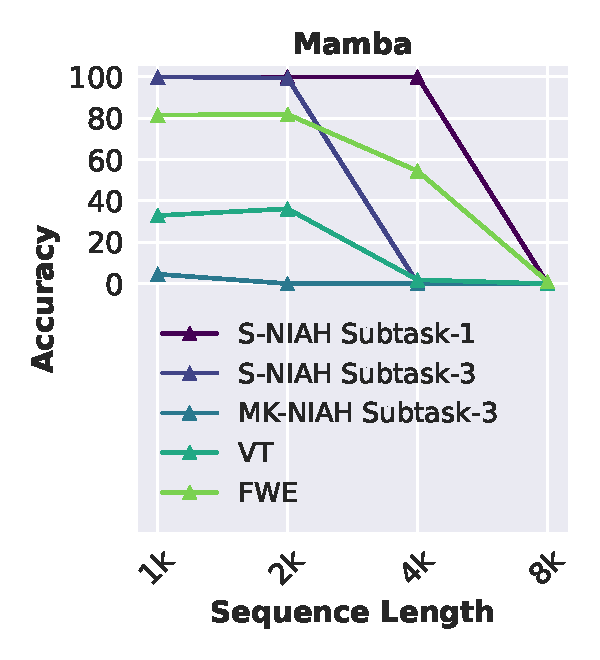
\includegraphics[width=0.3\linewidth]{Image/pdf/Mamba.pdf}
    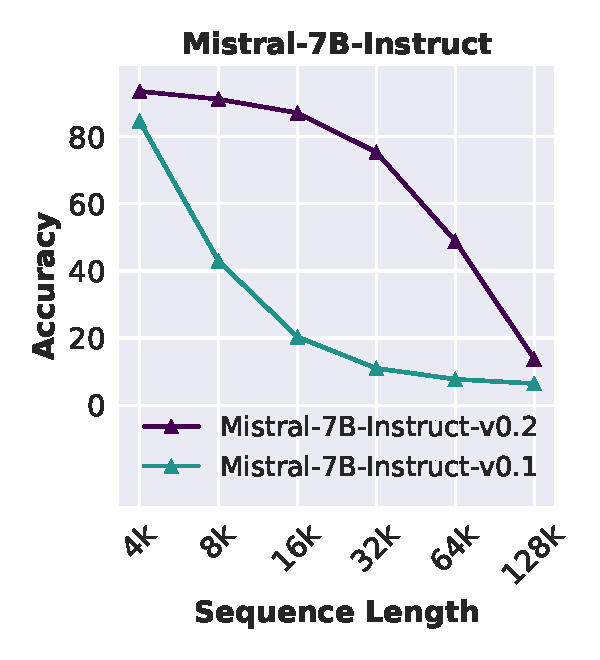
\includegraphics[width=0.3\linewidth]{Image/pdf/Mistral.pdf}
    \caption{TBD. \sscomment{contrast with mistralv2}}
    \label{fig:mamba-mistral}
\end{figure*}
% \paragraph{Sliding window attention model: Mistral-7B-Instruct-v0.1} \sscomment{i just realized it's hard to make any conclusion about sliding window with mistral v1 and v2, because they differ much more than if using SWA or not. v2 may have also gone through better optimization processes}